\section{Актуальность темы}
\begin{frame}
    {Актуальность темы}
    
    В настоящее время тенденция бурного развития информационных технологий во всех сферах деятельности человека оказывает весомое влияние на нефтегазовый сектор страны. енные компании, представляющие собой сложные многоуровневые производственные системы, для своего устойчивого развития требуют постоянного развития информационных технологий.  
    
    Сегодня наблюдается  бурное развитие процесса «цифровизации» нефтегазовой отрасли. Одним из путей развития данного процесса является внедрение беспроводных технологий.
    
    
\end{frame}

\begin{frame}
    {Актуальность темы}
    Активное использование беспроводных сетей основывается на ряде их преимуществ по сравнению с кабельными сетями:
    \begin{itemize}
        \item возможность получения информации с любой точки контролируемой территории;
        \item быстрый ввод в эксплуатацию по системе подключение типа Plug-\&-Play;
        \item сокращение капитальных затрат на создание сети; 
        \item уменьшение затрат на эксплуатацию;
        \item высокая гибкость, мобильность, масштабируемость;
        \item упрощенные требования к обслуживанию оборудования.
    \end{itemize}

  
\end{frame}

\section{Научно-техническая проблема}
\begin{frame}
    {Научно-техническая проблема}

    В рамках этого процесса возникает актуальная научно - техническая проблема \textbf{повышения качества проектирования беспроводной сети связи}, осуществляющей сбор и передачу информации в центр  управления с множества контролируемых объектов на некоторой территории. 

\end{frame}


\begin{frame}
    {Научно-техническая проблема}
    Процесс проектирования енной беспроводных сетей связи (БШС) состоит из последовательного решения взаимосвязанных задач:
    
    \bigskip

    \begin{itemize}
        \item выбор типов технических средств и протоколов;
        \item выбор топологической структуры сети;
        \item анализ и оптимизация пропускной способности каналов связи, маршрутизация информационных потоков и др.
    \end{itemize}

    \bigskip
    
    Задача \textbf{синтеза топологии} при комплексном проектировании БШС является основной проблемой исследования в данной работе.

\end{frame}

\begin{frame}
    {Научно-техническая проблема}

    \textbf{\underline{Объектом исследования}} БШС специальных типов, широко представленных на практике:
    
    \bigskip

    \begin{itemize}
        \item БШС для контроля линейных траекторий;
        \item БШС с ячеистой топологией (mesh) для контроля объектов, рассредоточенных на некоторой территории.
    \end{itemize}

    \bigskip

    \textbf{\underline{Предметом исследования}} является синтез топологической структуры беспроводной широкополосной сети.

    \bigskip
    
    \textbf{\underline{Целью}} состоит в разработке моделей и методов оптимального размещения базовых станций для БШС указанных типов, определяющего топологию таких сетей.
\end{frame}

\section{Положение 1}
\begin{frame}
    \begin{center}
        {Положение 1 - математические модели в виде задачи ЦЛП и экстремальной комбинаторной задачи для оптимального размещения базовых станций при проектировании БШС с линейной топологией}
    \end{center}
\end{frame}

\begin{frame}
    {Технологическая постановка задачи} 

    Для контроля над заданным линейным участком необходимо разместить базовые приемопередающие устройства (станции) таким образом, чтобы максимизировать покрытие с обеспечением условий технических и бюджетных ограничений. 

    \bigskip
    
    Постановка
    \begin{itemize}
        \item в виде задачи ЦЛП;
        \item в виде комбинаторной модели в экстремальной форме.
    \end{itemize}

\end{frame}

\begin{frame}
    Важно обеспечить связь любой станции со шлюзами на концах участка через систему размещенных станций. Задано множество станций
\end{frame}

\begin{frame}
    {задача ЦЛП}

    % Задаче в виде ЦЛП формулируется следующим образом. 

    \bigskip

    Задано множество станций $S = \{s_j\}$. Каждой станции приписаны параметры $s_j = \{r_j, \{R_{jq}\}, c_j \}$, $j = \overline{1,m}; q = \overline{1,m}; q \neq j$. 
    \begin{itemize}
        \item $r_j$ -- радиус покрытия станции,
        \item $R_{jq}$ -- это радиус связи между станцями $s_j$ и $s_q$,
        \item $c_j$ -- это стоимость.
    \end{itemize} 
    
    \bigskip

    Задан линейный участок длиной $L$ с концами в точка $a_0$ и $a_{n+1}$. 
    
    Внутри  отрезка $[a_0, a_{n+1}]$ задано конечное множество точек $A=\{a_i\}, i=\overline{1,n}$; эти точки соответствуют набору свободных мест, где могут быть размещены станции.
    
    Каждая точка $a_i$ определяется своей одномерной координатой $l_i$. 
    
    \bigskip
    
    Заданы станции специального вида $s_{m+1}$ -- шлюзы. Данные шлюзы размещены на концах $a_0$ и $a_{n+1}$ данного линейного участка. Для данных станций параметр радиуса покрытия $r_{m+1}=0$. Радиус связи и стоимость не заданы.
    \bigskip

\end{frame}



\begin{frame}
    \frametitle{задача ЦЛП}
    \begin{minipage}[t]{1\linewidth}
        \fontsize{8pt}{7.2}\selectfont
        Целевая функция:
        \begin{equation}
        f =  \sum\limits_{i=1}^n (y_i^- + y_i^+) \rightarrow max,
        \end{equation}

        где $y_i^+$ и $y_i^-$ , $i= \overline{0,n+1}$ определяют охват покрытия (справа и слева, соответственно) станций.
        \bigskip
    \end{minipage}

    \begin{minipage}[t]{0.5\linewidth} 
        \fontsize{8pt}{7.2}\selectfont
        Каждая станция должна быть размещена только в одной точке:
            
        \begin{equation}
        \label{eq:part3_xij}
        \sum\limits_{j=1}^n x_{ij} \leq 1, \quad j = \overline{1,m}. 
        \end{equation}
        
        % Значения покрытий не превышают радиус покрытия станции, размещенной в точке $ a_i $, и равны 0, если в точке $a_i$  нет станции \cref{eq:part3_yi_1, eq:part3_yi_2}:
        
        
        \begin{equation}
        \label{eq:part3_yi_1}
        y_i^+ \leq \sum\limits_{j=1}^m x_{ij} \cdot r_j, \quad i = \overline{1,n};
        \end{equation}
        
        \begin{equation}
        \label{eq:part3_yi_2}
        y_i^- \leq \sum\limits_{j=1}^m x_{ij} \cdot r_j, \quad i = \overline{1,n}. 
        \end{equation}

        $$
            x_{ij} = 
             \begin{cases}
               1& \text{, станция $s_j$, размещенная на точке $a_i$,} \\
               0 & \text{, в противном случае.}
             \end{cases}
        $$

    \end{minipage}
    \hfill
    \begin{minipage}[t]{0.4\linewidth}
        
        \center{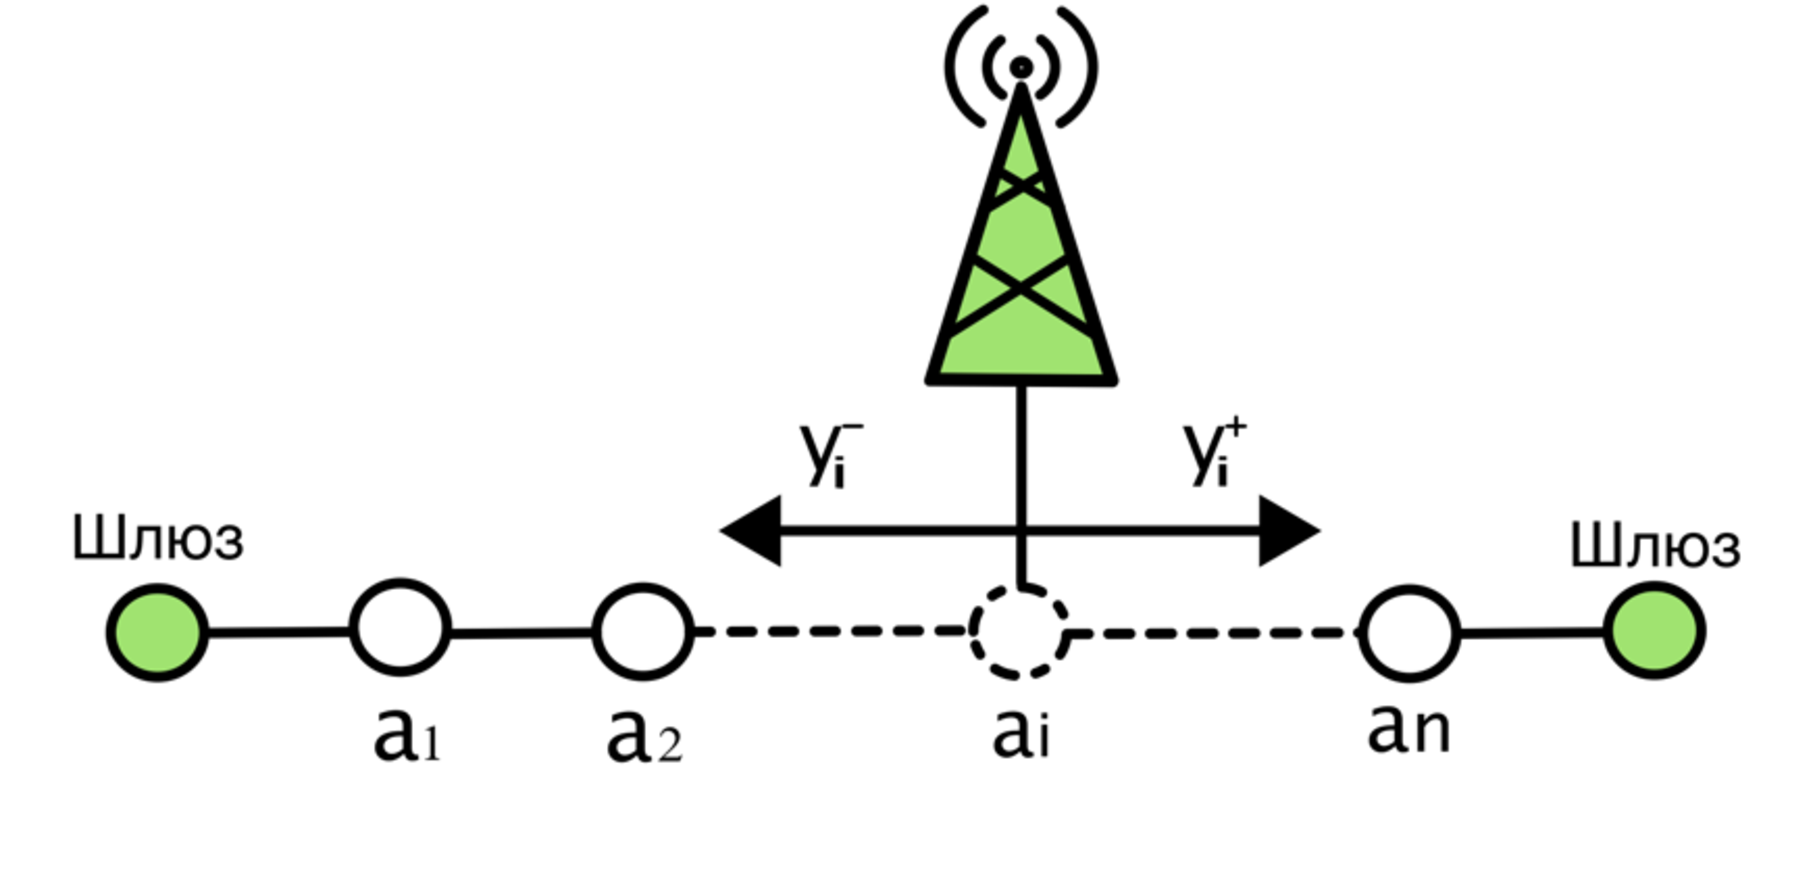
\includegraphics[scale=0.15]{station_coverage.pdf}}
        \center{\textbf{Охват покрытия станции}}
    \end{minipage}

    % \bigskip
    % \fontsize{8pt}{7.2}\selectfont
    % где $y_i^+$ и $y_i^-$ , $i= \overline{0,n+1}$ определяют охват покрытия (справа и слева, соответственно) станций.


\end{frame}

\begin{frame}
    \frametitle{задача ЦЛП}
    \begin{minipage}[t]{0.5\linewidth}
        \begin{equation}
            \label{eq:part3_ei}
            e_i =  \sum\limits_{j=1}^m x_{ij}, \quad i = \overline{1,n}. 
          \end{equation}
    \end{minipage}

    \begin{minipage}[t]{0.5\linewidth}
        % \fontsize{8pt}{7.2}\selectfont
        
    \bigskip
    \bigskip
    \bigskip
    Суммарное покрытие между двумя станциями не больше расстояния между ними.
          
        %   Каждая станция должна быть размещена только в одной точке. \cref{eq:part3_xij}:
          
        %   \begin{equation}
        %     \label{eq:part3_xij}
        %     \sum\limits_{j=1}^n x_{ij} \leq 1, \quad j = \overline{1,m}. 
        %   \end{equation}
          
        %   Значения покрытий не превышают радиус покрытия станции, размещенной в точке $ a_i $, и равны 0, если в точке $a_i$  нет станции \cref{eq:part3_yi_1, eq:part3_yi_2}:
          
          
        %   \begin{equation}
        %     \label{eq:part3_yi_1}
        %     y_i^+ \leq \sum\limits_{j=1}^m x_{ij} \cdot r_j, \quad i = \overline{1,n};
        %   \end{equation}
          
        %   \begin{equation}
        %     \label{eq:part3_yi_2}
        %     y_i^- \leq \sum\limits_{j=1}^m x_{ij} \cdot r_j, \quad i = \overline{1,n}. 
        %   \end{equation}
          
        %   Общая область покрытия между любыми двумя точками $ a_i $ и $ a_k $, где расположены станции, не может превышать расстояние между этими точками \cref{eq:part3_yi_3, eq:part3_yi_4}.
          
        %   \begin{equation}
        %     \label{eq:part3_yi_3}
        %     y_i^+ + y_k^- \leq \frac{l_k - l_i}{2} \cdot (e_i + e_k ) + (2 - e_i - e_k ) \cdot L, \quad i = \overline{1,n},  \quad k = \overline{i+1,n+1};
        %   \end{equation}
          
        %   \begin{equation}
        %     \label{eq:part3_yi_4}
        %     y_i^- + y_k^+  \leq \frac{l_i-l_k}{2} \cdot (e_i + e_k) + (2 - e_i - e_k) \cdot L, \quad i = \overline{1,n}, \quad k = \overline{i-1,0},
        %   \end{equation}
        %   где $ l_k $ и $ l_i $ - координаты точек $ a_i $ и $ a_k $, соответственно. Это условие исключает влияние пересечений покрытий станций при вычислении общего значения покрытия между станциями (Рис. \cref{fig:part3_total_coverage_between_points}).
          
    

    \end{minipage}
    \hfill
    \begin{minipage}[t]{0.47\linewidth}
        
        \center{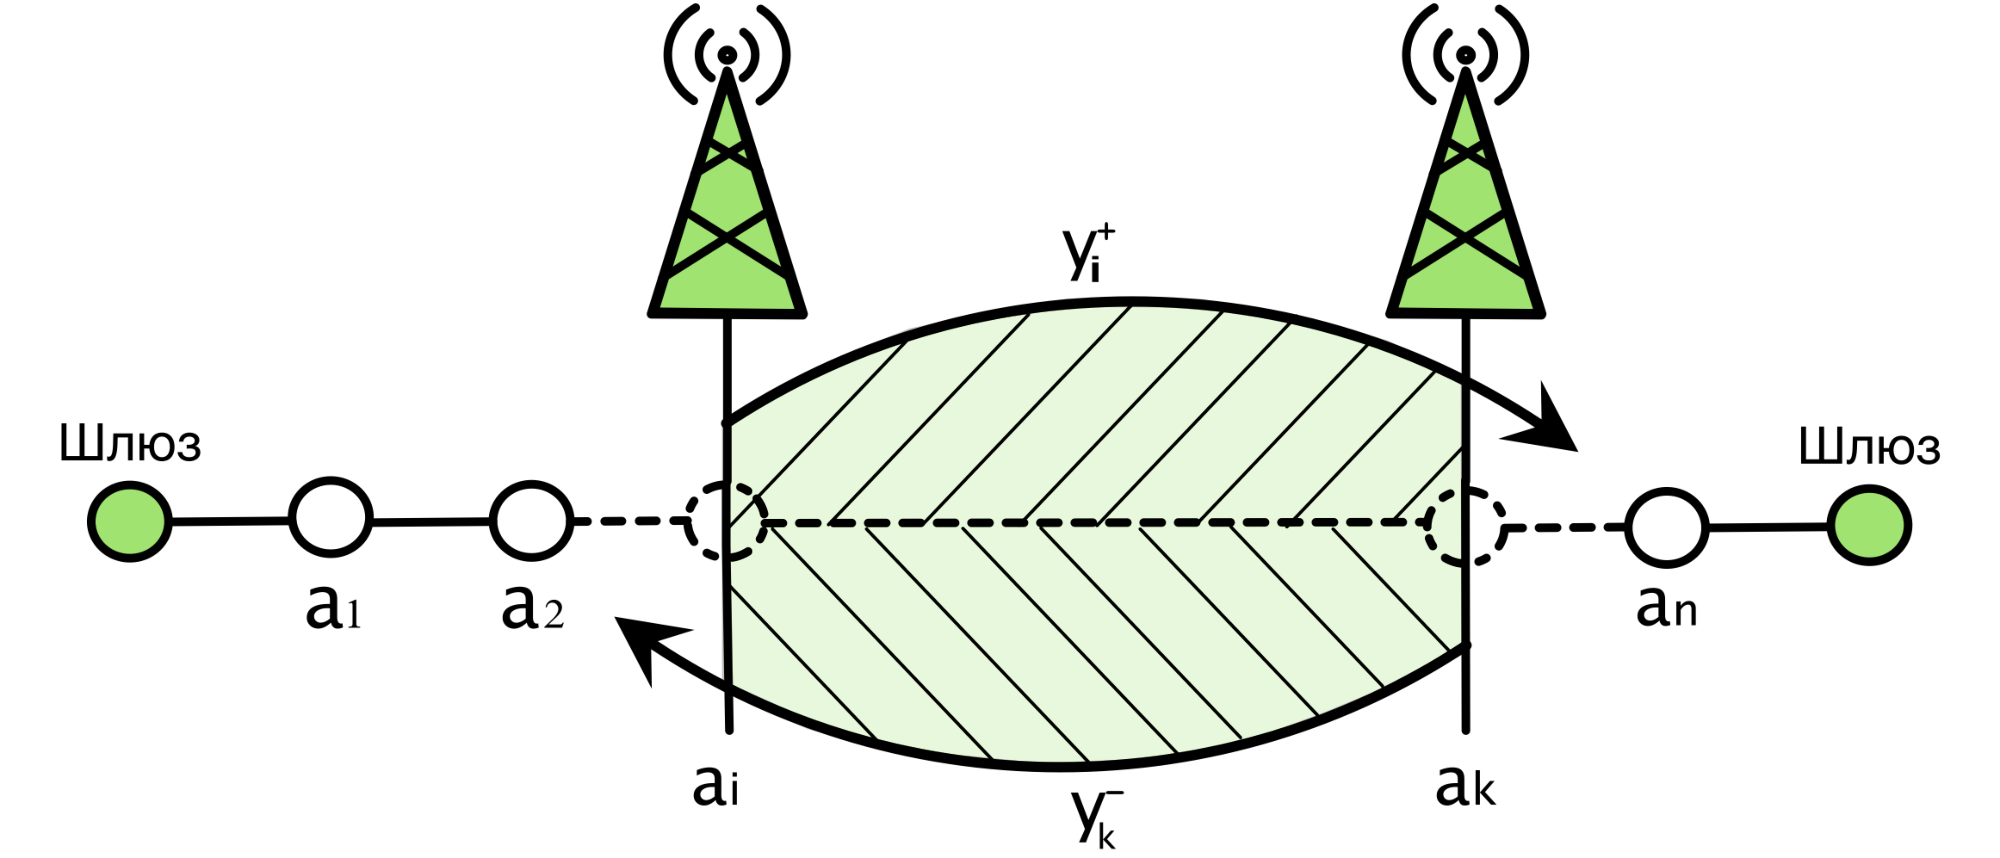
\includegraphics[scale=0.15]{total_coverage_between_points.pdf}}
        \center{\textbf{Покрытие между станцями}}
    \end{minipage}

    \bigskip
    \fontsize{8pt}{7.2}\selectfont
    \begin{equation}
        \label{eq:part3_yi_3}
        y_i^+ + y_k^- \leq \frac{l_k - l_i}{2} \cdot (e_i + e_k ) + (2 - e_i - e_k ) \cdot L, \quad i = \overline{1,n},  \quad k = \overline{i+1,n+1};
      \end{equation}
      
      \begin{equation}
        \label{eq:part3_yi_4}
        y_i^- + y_k^+  \leq \frac{l_i-l_k}{2} \cdot (e_i + e_k) + (2 - e_i - e_k) \cdot L, \quad i = \overline{1,n}, \quad k = \overline{i-1,0},
      \end{equation}


\end{frame}

\begin{frame}
    \frametitle{Разделяющие линии}
    \begin{minipage}[c]{0.47\linewidth}
        \center{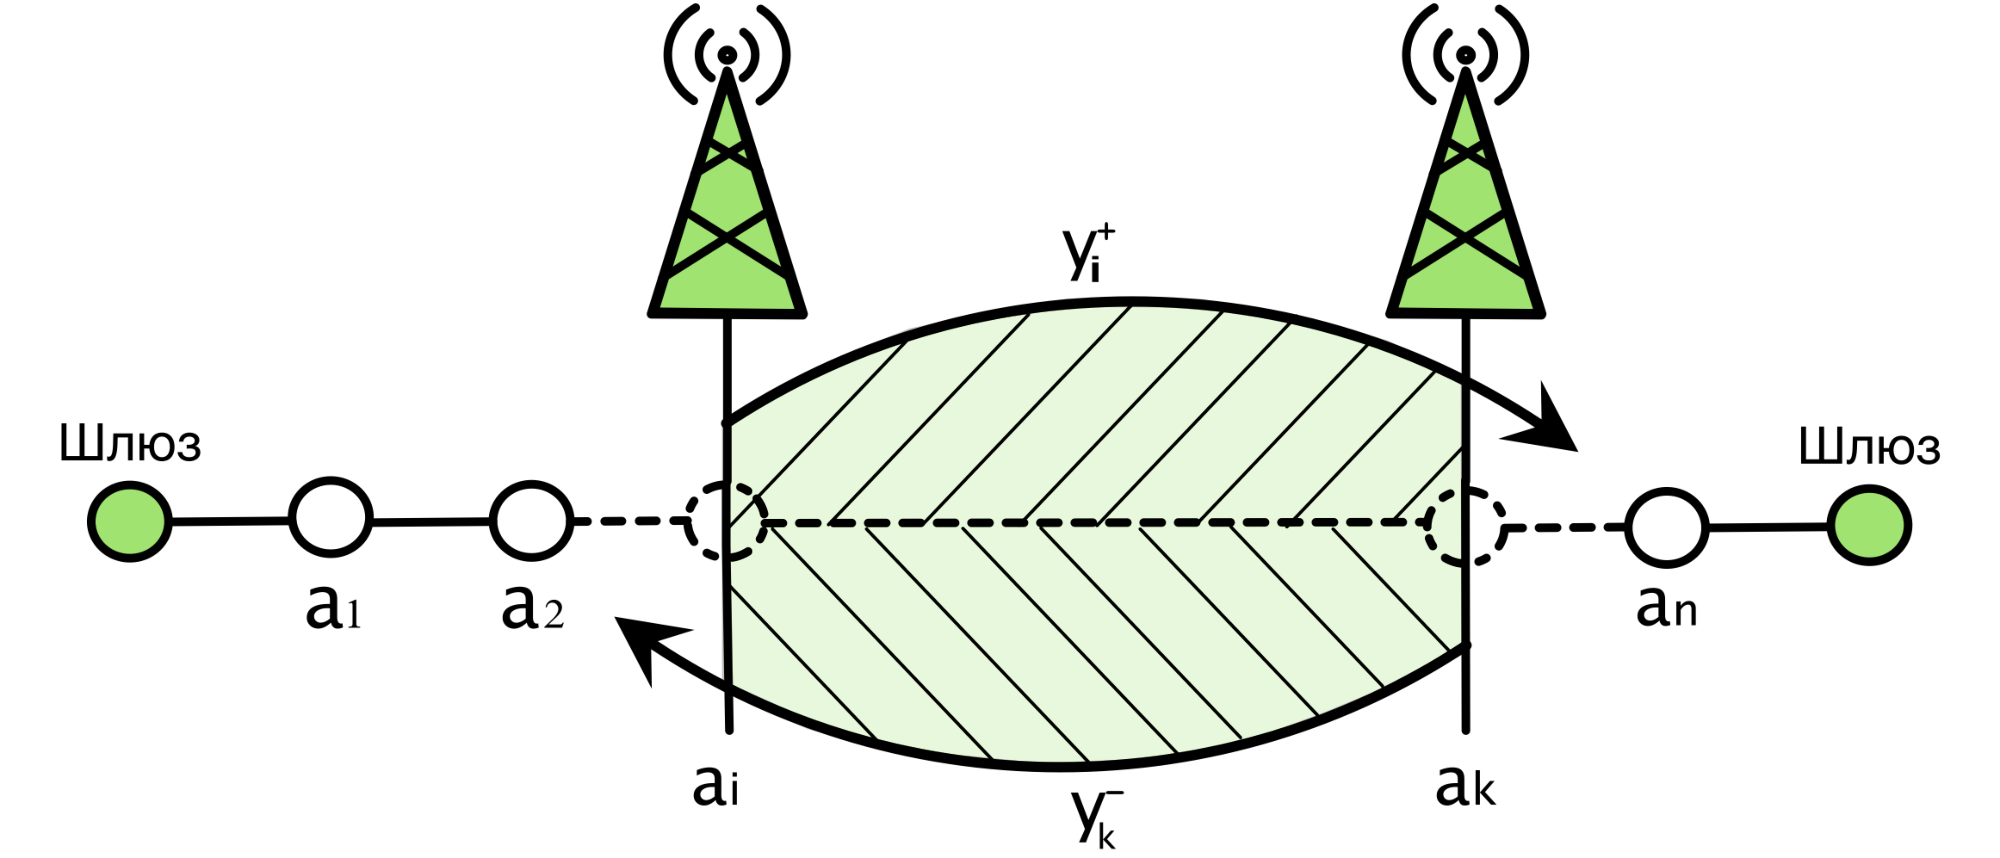
\includegraphics[scale=0.15]{total_coverage_between_points.pdf}}
        
        \bigskip
        \hrule{}
        \bigskip
        \textbf{Составная \\ подпись 1}
    \end{minipage}
    \hfill
    \vrule{}
    \hfill
    \begin{minipage}[c]{0.47\linewidth}
        \flushright
        \textbf{Составная \\ подпись 2}
        \center{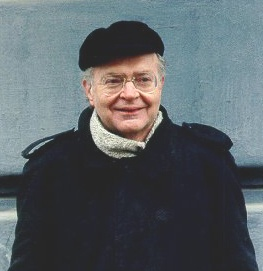
\includegraphics[width=1\linewidth]{knuth2}}
    \end{minipage}
\end{frame}

\begin{frame}

\end{frame}

\subsection{Нумерованные}

\begin{frame}
    \frametitle{Нумерованные списки}
    \begin{enumerate}
        \item один
        \item два
        \item три
    \end{enumerate}
\end{frame}
\note{
    Этот текст будет виден только если его отображение включено
    в~файле \textbf{Presentation/setup}.
    Для раздельного вывода презентации и заметок на~разные экраны (как
    в~impress или powerpoint) можно использовать программу
    \textit{pdf-presenter-console}.
}

\subsection{Не нумерованные}


\begin{frame}
    \frametitle{Перечисления}
    \begin{itemize}
        \item Проблема 1
        \item Проблема 2
        \item Проблема 3
    \end{itemize}
\end{frame}
\note[itemize]{
    \item Тезис 1
    \item Тезис 2
    \item Тезис 3
}

\subsection{Комбинированные}

\begin{frame}
    \frametitle{Комбинация списков}
    \begin{enumerate}
        \item \textbf{Задача 1}
              \begin{itemize}
                  \item Подзадача 1-1
                  \item Подзадача 1-2
              \end{itemize}
        \item \textbf{Задача 2}
              \begin{itemize}
                  \item Подзадача 2-1
                  \item Подзадача 2-2
                  \item Подзадача 2-3
              \end{itemize}
        \item \textbf{Задача 3}
              \begin{itemize}
                  \item Подзадача 3-1
                  \item Подзадача 3-2
                  \item Подзадача 3-3
              \end{itemize}
    \end{enumerate}
\end{frame}
\note[itemize]{
    \item Задача 1
    \item Задача 2
    \item Задача 3
}

\begin{frame}[allowframebreaks]
    \frametitle{Разделение слайда}
    Поясняющий текст
    \begin{itemize}
        \item Один
        \item Два
        \item Три
    \end{itemize}
    \framebreak
    Продолжение предыдущего слайда
\end{frame}

\section{Графика}
\begin{frame}[plain, noframenumbering]
    \begin{center}
        \Huge
        Графика
    \end{center}
\end{frame}


\begin{frame}
    \frametitle{Одиночное изображение}
    \centering
    
\includegraphics[width=0.8\linewidth]{latex} % окружение figure не требуется
\end{frame}

\begin{frame}
    \frametitle{Векторная графика}
    \begin{figure}
        \centering
        \ifdefmacro{\tikzsetnextfilename}{\tikzsetnextfilename{tikz_presentation}}{}% присваиваемое предкомпилированному pdf имя файла (не обязательно)
        \begin{tikzpicture}
  \draw[<->,thick] (0,6) -- (0,0) -- (10,0); % axis
  \draw[help lines] (3,0) -- (3,5); % fill end
  \draw[help lines] (6,0) -- (6,5); % flattop end
  \draw[help lines] (9,0) -- (9,5); % decay end
  \draw[<->, thin] (0,5) -- (3,5); % fill
  \draw[<->, thin] (3,5) -- (6,5); % flattop
  \draw[<->, thin] (6,5) -- (9,5); % decay
  \draw[blue, ultra thick] (0,0) -- (0,4) -- (6,4) -- (6,0); % power
  \draw[red, ultra thick, domain=0:3] plot (\x, {4*(1 - exp(-1.5*\x))}); % fill plot
  \draw[red, ultra thick, domain=3:6] plot (\x, {4*(1 - exp(-1.5*\x))}); % flattop plot
  \draw[red, ultra thick, domain=6:9.5] plot (\x, {4*(1 - exp(-9)) - 4*(1 - exp(-1.5*\x+9))}); % decay plot
  \node [above] at (0,6) {\(E_{acc}\)};
  \node [right] at (10,0) {\(t\)};
  \node at (1.5,5.4) {заполнение};
  \node at (4.5,5.4) {работа};
  \node at (7.5,5.4) {затухание};
  \node at (4.5,1.4) {пучки};
  \foreach \x in {3.1,3.3,...,5.9} {
    \draw[->, green, thick] (\x,0) -- (\x,1);
  }
\end{tikzpicture}
    \end{figure}
\end{frame}

\subsection{Расположение}

\begin{frame}
    \frametitle{Изображения по-вертикали}
    \centering
    \vfill
    
\includegraphics[width=0.8\linewidth,height=0.1\textheight]{latex} \\
    \TeX
    \vfill
    
\includegraphics[width=0.8\linewidth,height=0.2\textheight]{latex} \\
    \LaTeX
    \vfill
    
\includegraphics[scale=0.2]{latex} \\
    \vfill
\end{frame}


\begin{frame}
    \frametitle{Изображения по-горизонтали}
    \begin{minipage}[t]{0.47\linewidth}
        \textbf{Составная \\ подпись 1}
        \center{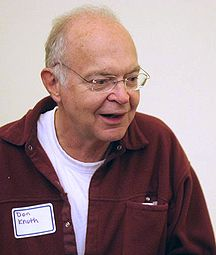
\includegraphics[width=1\linewidth]{knuth1}}
    \end{minipage}
    \hfill
    \begin{minipage}[t]{0.47\linewidth}
        \textbf{Составная \\ подпись 2}
        \center{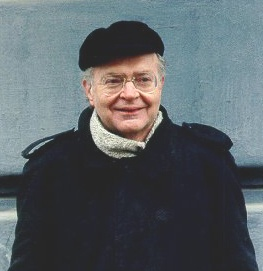
\includegraphics[width=1\linewidth]{knuth2}}
    \end{minipage}
\end{frame}

\subsection{Линии}

\begin{frame}
    \frametitle{Разделяющие линии}
    \begin{minipage}[c]{0.47\linewidth}
        \center{
\includegraphics[width=1\linewidth]{latex}}
        \bigskip
        \hrule{}
        \bigskip
        \textbf{Составная \\ подпись 1}
    \end{minipage}
    \hfill
    \vrule{}
    \hfill
    \begin{minipage}[c]{0.47\linewidth}
        \flushright
        \textbf{Составная \\ подпись 2}
        \center{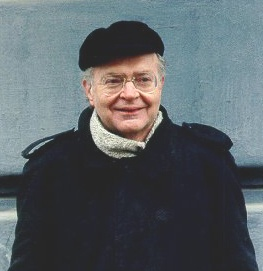
\includegraphics[width=1\linewidth]{knuth2}}
    \end{minipage}
\end{frame}

\section{Остальное}
\begin{frame}[plain, noframenumbering]
    \begin{center}
        \Huge
        Остальное
    \end{center}
\end{frame}

\subsection{Формулы}

\begin{frame}
    \frametitle{Формулы}
    \[
    \left\{
    \begin{array}{rl}
        \dot x = & \sigma (y-x)  \\
        \dot y = & x (r - z) - y \\
        \dot z = & xy - bz
    \end{array}
    \right.
    \]
\end{frame}

\begin{frame}
    \frametitle{amsmath}
    \centering
    \begin{minipage}[t]{0.5\linewidth}
        \begin{multline*}
            y = 1 x^1 + 2 x^2 + 3 x^3 + \\ + 4 x^4 + 5 x^5 + \dots
        \end{multline*}
    \end{minipage}
\end{frame}

\begin{frame}[allowframebreaks]
    \frametitle{Уравнения Максвелла}
    \centering{
        \small
        \def\arraystretch{1.8}%
        \begin{tabular}{ll}
            \toprule
            Интегральная форма                                                                                                                                            & Дифференциальная форма                                                          \\ \midrule
            \(Q_e(t) = \displaystyle\oiint_S \vec D(t) \cdot d\vec{s} = \displaystyle\iiint_V \rho_v(t) dv\)                                                              & \(\nabla \cdot \vec D(t) = \rho_v(t)\)                                          \\
            \(\displaystyle\oiint_S \vec B(t) \cdot d\vec{s} = 0\)                                                                                                        & \(\nabla \cdot \vec B(t) = 0\)                                                  \\
            \(V_{emf}(t) = \displaystyle\oint_L \vec E(t) \cdot d\vec{l}\) = \(- \displaystyle\iint_S \left[\frac{\partial\vec{B}(t)}{\partial t}\right] \cdot d\vec{s}\) & \(\nabla \times \vec E(t) = - \frac{\partial\vec{B}(t)}{\partial t}\)           \\
            \(I(t) = \displaystyle\oint_L \vec H(t) \cdot d\vec{l} = \displaystyle\iint_S \left[\vec J(t) + \frac{\partial\vec{D}(t)}{\partial t}\right] \cdot d\vec{s}\) & \(\nabla \times \vec H(t) = \vec J(t) + \frac{\partial\vec{D}(t)}{\partial t}\) \\ \midrule
            \(\displaystyle\oiint_S \vec J \cdot d\vec{s} = -\frac{\partial Q_e}{\partial t}\)                                                                            & \(\nabla \cdot \vec J = - \frac{\partial \rho_v}{\partial t}\)                  \\
            \bottomrule
            \multicolumn{2}{c}{\(\vec D(t) = \left[\varepsilon(t)\right] * \vec E(t)\)}                                                                                                                                                                     \\
            \multicolumn{2}{c}{\(\vec B(t) = \left[\mu(t)\right] * \vec H(t)\)}                                                                                                                                                                             \\
        \end{tabular}
    }
    \framebreak

    \hspace{0.05\linewidth}
    \centering{
        \small
        \def\arraystretch{1.8}%
        \begin{tabular}{ll}
            \toprule
            Интегральная форма                                                                                                                & Дифференциальная форма                               \\ \midrule
            \(Q_e = \displaystyle\oiint_S \vec D \cdot d\vec{s} = \displaystyle\iiint_V \rho_v dv\)                                           & \(\nabla \cdot \vec D = \rho_v\)                     \\
            \(\displaystyle\oiint_S \vec B \cdot d\vec{s} = 0\)                                                                               & \(\nabla \cdot \vec B = 0\)                          \\
            \(V_{emf} = \displaystyle\oint_L \vec E \cdot d\vec{l}\) = \(- \displaystyle\iint_S \left[j \omega \vec B\right] \cdot d\vec{s}\) & \(\nabla \times \vec E = - j \omega \vec B\)         \\
            \(I = \displaystyle\oint_L \vec H \cdot d\vec{l} = \displaystyle\iint_S \left[\vec J + j \omega \vec D\right] \cdot d\vec{s}\)    & \(\nabla \times \vec H = \vec J + j \omega \vec{D}\) \\ \midrule
            \(\displaystyle\oiint_S \vec J \cdot d\vec{s} = - j \omega Q_e\)                                                                  & \(\nabla \cdot \vec J = - j \omega \rho_v\)          \\
            \bottomrule
            \multicolumn{2}{c}{\(\vec D(t) = \left[\varepsilon\right] \vec E(t)\)}                                                                                                                   \\
            \multicolumn{2}{c}{\(\vec B(t) = \left[\mu\right] \vec H(t)\)}                                                                                                                           \\
        \end{tabular}
    }
\end{frame}

\subsection{Таблицы}

\begin{frame}
    \frametitle{Таблица}
    \centering
    \begin{tabular}{|l|l|}
        \hline
        \textbf{Заголовок 1} & \textbf{Заголовок 2} \\
        \hline
        Сумма                & \(b+a\)              \\
        \hline
        Разность             & \(a-b\)              \\
        \hline
        Произведение         & \(a*b\)              \\
        \hline
    \end{tabular}
\end{frame}

\begin{frame}
    \frametitle{Другая таблица}
    \centering
    \begin{tabular}{lc}
        \toprule
        \multicolumn{1}{c}{\textbf{Заголовок 1}} & \textbf{Заголовок 2} \\ \midrule
        Сумма                                    & \(b+a\)              \\
        Разность                                 & \(a-b\)              \\
        Произведение                             & \(a*b\)              \\
        \bottomrule
    \end{tabular}
\end{frame}


\subsection{Разное}

\begin{frame}
    \frametitle{Большой многоуровневый список}
    \begin{itemize}
        \item \textbf{Пункт 1}
              \begin{itemize}
                  \itemi Подпункт 1-1
                  \itemi Подпункт 1-2
              \end{itemize}
        \item \textbf{Пункт 2}
              \begin{itemize}
                  \itemi Подпункт 2-1
              \end{itemize}
        \item \textbf{Пункт 3}
              \begin{itemize}
                  \itemi Подпункт 3-1
                  \itemi Подпункт 3-2
              \end{itemize}
        \item \textbf{Пункт 4}
              \begin{itemize}
                  \itemi Подпункт 4-1
              \end{itemize}
        \item \textbf{Пункт 5}
              \begin{itemize}
                  \itemi Подпункт 5-1
                  \itemi Подпункт 5-2
                  \itemi Подпункт 5-3
              \end{itemize}
    \end{itemize}
\end{frame}

\begin{frame}
    \frametitle{Четыре изображения}
    \centering
    
\includegraphics[width=0.35\linewidth,angle=35]{latex}
    
\includegraphics[width=0.35\linewidth,angle=135]{latex}\\
    
\includegraphics[width=0.35\linewidth,angle=15]{latex}
    
\includegraphics[width=0.35\linewidth,angle=-15]{latex}
\end{frame}

